\clearpage
\section{Oblivious Transfer with Discrete Variables}

\begin{tcolorbox}	
\begin{tabular}{p{2.75cm} p{0.2cm} p{10.5cm}} 	
\textbf{Student Name}  &:& Mariana Ramos\\
\textbf{Starting Date} &:& September 18, 2017\\
\textbf{Goal}          &:& Oblivious transfer implementation with discrete variables.
\end{tabular}
\end{tcolorbox}

Oblivious transfer is one of the most fundamental basics in Cryptography and it is used in a number of communication protocols in order to guarantee its security against eavesdropping. This one-out-of-two Oblivious Transfer Protocol consists in a communication protocol between Alice and Bob which has two classical channels and one quantum communication channel. At the beginning of the protocol Alice has two messages $m_1$ and $m_2$ and Bob wants to read one of them thereby choosing a random bit b, and in this way he will learn the message $m_{b}$. Two conditions must be fulfilled:
\begin{enumerate}
	\item{The protocol must be concealing, i.e at the beggining of the protocol Bob does not know nothing about the messages sent by Alice, while at the end of the protocol Bob will learn the message b chose by him.}
	\item{The protocol is oblivious, i.e at the end of the protocol Alice remains without learning which message was choosen by Bob. Alice cannot learn anything about bit b and Bob cannot learning nothing about the other message $m_{1-b}.$}
\end {enumerate}

\subsection{OT protocol detailed}
In this case study, an OT protocol will be implemented as described bellow. 

Let $U=\{+,\times\}^{n} \times \{0,1\}^{n}$ where $+$ and $\times$ are the rectilinear and diagonal basis, respectively.
A first phase of the protocol is to test Bob's honesty.
\begin{enumerate}
	\item{Alice picks a random $u=(a,g) \in U$ for each photon \textit{i}, where $\textbf{a[i]}$ represents the basis and $\textbf{g[i]}$ the state. Then, Alice sens to Bob the photons \textit{i} (where $0\le i \le n$) with polarizations given by $a[i]$ and $g[i]$.}
	\item{Bob randomly chooses $b \in {+, \times}^{n}$ and then he measures the photons \textit{i} in basis $b[i]$ and records the data in an array $h[i] \in {0,1}$. He makes a commit of all \textit{n} pairs $(b[i],g[i])$ to Alice.}
	\item{Alice randomly chooses a subset $R \subseteq {1,2,...,n}$ and tests some positions in this set with  the pair commited by Bob. If any \textit{i} reveals $a[i]=b[i]$ and $g[i] \neq h[i]$ Alice immediately stops the protocol, otherwise she accepts the commitment and the protocol continue.}
\end{enumerate}

At this time, we can assume that Bob is honest. Let two new sets, $T_{0}$ the set of all $0\le i \le n$ with $a[i]=b[i]$, and $T_{1}$ the set of all  $0\le i \le n$ with $a[i]\neq b[i]$.
\begin{enumerate}
	\item{First, Alice sends through a classical channel the basis \textbf{a} to Bob.}
	\item{Bob chooses two subsets $I_{0}$ and $I_{1}$ which represents the set of positions which Bob was wrong and the positions he has succeeded, respectively. He send through a classical channel this subsets in a random order, $\{ I_{0},I_{1} \}$ or $\{ I_{1},I_{0} \}$.}
	\item{Alice send to Bob the two messages encrypted.}
	\item{Bob receives the two messages, though he only may has learnt one of them.}
\end{enumerate}

\subsection{A more concrete example about OT-protocol}

Let's look in a more specific example. Let $m_{1}: [1 1 0]$ and $m_{2}:[0 0 1]$ the two messages sent by Alice. First of all, Alice picks a random $g[i]$ which is the state and a random basis $a[i]$, being \textit{i} the photon's position.

\begin{table}[H]
\centering
\begin{tabular}{c|c|c|c|c|c|c|c}
\textbf{\textit{i}}         & 1 & 2 & 3 & 4 & 5 & 6      \\ \hline
\textbf{\textit{Data}}  & 0 & 1 & 0 & 1 & 1 & 1     \\ \hline
\textbf{\textit{Alice's basis}} & + & + & $\times$ &+ & $\times$ & $\times$ \\ \hline
\textbf{\textit{Bob's basis}} & $\times$ & + & + &+ & $\times$ & + \\ \hline

		 & \underline{0} & 1 & \underline{1} & 1 & 1 & \underline{0} \\ \hline
\end{tabular}
\end{table}

The data sent by Alice is encrypted one bit for two, i.e if Alice sends 00 or 11 means the bit is zero, otherwise if she sends 01 or 10 means the bit is 1. It is useful against eavesdropping, since if he or she only knows one of the bits, it is impossible knows which bit is.
After Alice made her choices, Bob picks a random basis too. When Alice sends her choice, Bob knows in which positions he has succeeded and then he will pick two new sets:

\begin{center}
$I_{0} \{ 1,3,6 \}$ - Positions of wrong choices\\
$I_{1} \{ 2,4,5 \}$ - Positions of right choices
\end{center}

After that, Bob sends to Alice a new set $ \{ I_{0},I_{1} \}$ or $\{ I_{1}, I_{0}\}$ radonmly choosen. Alice receives $\{ I_{i}, I_{\bar{i}}\}$ and sends to Bob $\{ m_{1}, m_{2}\}$ encrypted:

$$m_{1} \oplus{} \{ 1 1 1 \} = \{ 0 0 1\}$$
$$m_{2} \oplus{} \{ 0 0 1 \} = \{ 0 0 0\}$$

After Bob received the encrypted messages from Alice, he only is able to desincrypted the message he wants, in this case message 1, as we can see bellow:
\begin{center}
$\{ 0 0 1\} \oplus{} \{ 1 1 1\} = \{ 1 1 0\} $: Message 1 $\surd$ \\
$\{ 0 0 0\} \oplus{} \{ 0 1 0\} = \{ 0 1 0\} $: Message 2 $\times$ \\
\end{center}

Bob only was able to learn one of the messages and Alice still does not know which message Bob has learnt.

\subsection{Experimental Setup}

In a first phase, this protocol will be simulatedand then a experimental setup will be built in laboratory.

In order to implement the protocol described above, the setup below will be built. 
\begin{figure}[H]
	\centering
	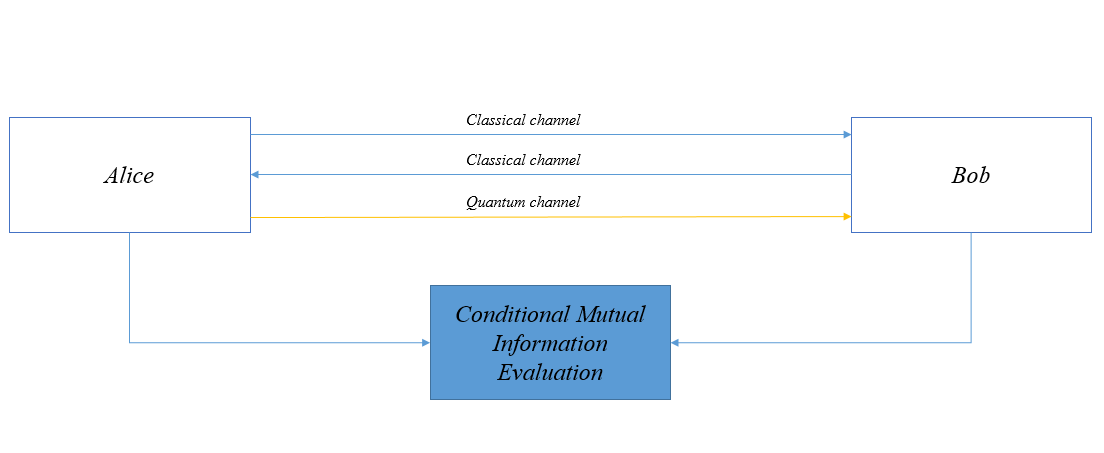
\includegraphics[width=1.0\textwidth, height=7cm]{./sdf/ot_with_discrete_variables/figures/SetupOt.png}
	\caption{Experimental Setup}\label{experimentalsetup}
\end{figure}

There must be two computers, one on Alice's side and other on Bob's side in order that they can communicate through classical channels. There will be three channels, two classical channels and one quantum channel. In \textit{Conditional Mutual Information Evaluation} block it qill be calculated $I(A,B|m_{i},i)$ and $I(A,B|m_{\bar{i}, i})$.
Alice send discrete photon through a quantum channel and the other two channels are for changing infomartion between Alice and Bob according with the above protocol.

